\chapter{Background\label{cha:background}}
%Provide background about the subject matter (e.g. How was morse code
%developed?  How is it used today?.

%This is a place where there are usually many citations.
%It is suspicious when there is not.
%Include the purpose of the different equipment and your design intent. 
%Include references to relevant scientific/technical work and books.
%What other examples of similar designs exist?
%How is your approach distinctive?

%If you have specifications or related standards, these must be
%described and cited also.  As an example, you might cite the specific
%RoboSub competition website (and documents) if working on the lighting system for an AUV\cite{guls2016auvlight}\index{AUV}
\section{Similar Designs}
Several products and projects exist which relate to our project. 
There is however no product or project that completely fulfills the needs of our customer. 
The following chapters cover the main features of the products and projects that can be useful for this project. 


\subsection{Permobil Smartdrive MX2+ Power Add-On Kit}
The Permobil Smartdrive MX2+ Power Add-On Kit is attached to wheelchairs, providing power assist for the user. 

\begin{figure}[!ht]
    \centering
    \includegraphics[height=50mm]{graphics/permobil.png}
    \caption{Permobil Smartdrive MX2+ Power Add-On Kit \cite{permobil_smartdrive_2022}.}
    \label{fig:permobil}
\end{figure}

It uses a 250W brushless dc motor to power the chair, giving it a maximum speed of 8.8 km/h and weighing only 5.7 kg for a user weight ranging from 14 to 150 kg.
Figure \ref{fig:permobil} shows the Permobil attached to a wheelchair. 
The user can turn the power assist on by using a wristband, PushTracker E2. 
The user can also change the speed settings and review system usage in the PushTracker E2. 
Permobil comes with a Switch Control, that can be adjusted to the user, which can provide momentary burst of power or  consistent power over extended distances \cite{permobil_smartdrive_2022}. 


\subsection{Airwheel SR5}
The Airwheel SR5 is a smart following suitcase. 
It uses UWB high-accuracy location technology to track the smart band the user has on, recognizing the distance between the user and suitcase.
It has two modes; auto-follow mode, and normal tow mode. 
If the suitcase is in auto-follow mode, it will draw up the motor, using 20W motor, to protect it and make it easy for the user to tow the luggage.
The SR5 has bluetooth 4.0, so it can be connected to the users smartphone, making it easy for the user to change settings like changing speed and to drive the suitcase manually. 
To detect obstacles it uses ultrasonic infrared sensor and plans dynamically to avoid them. 
It can reach up to 6 km/h with two 50 W motors, rated at speed 500 rpm. 
The SR5 is powered by a lithium-ion battery which weighs 340g and battery capacity of 62.6Wh.
The total weight of the suitcase is 6kg. 
The Airwheel SR5 can be seen in figure \ref{fig:airwheelsr5} along with the smart band \cite{airwheel_functions_2022}. 

\begin{figure}[!ht]
    \centering
    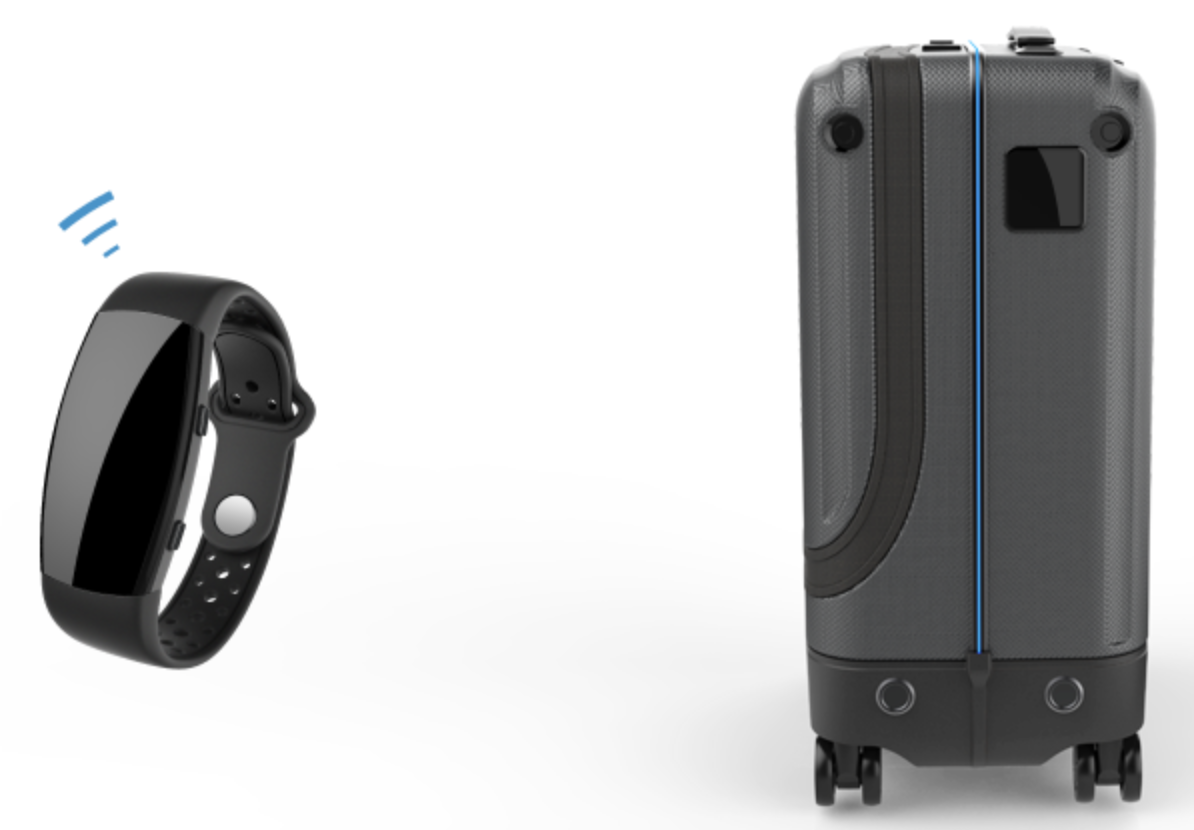
\includegraphics[height=50mm]{graphics/airwheel_sr5.png}
    \caption{Airwheel SR5 along with the Smart Band \cite{airwheel_functions_2022}.}
    \label{fig:airwheelsr5}
\end{figure}



\subsection{Robotic Wheelchair with Omni-directional vision}
This wheelchair was a project done at Saitama University and can the overview of the chair be seen in figure \ref{fig:omni-chair}. 
The robotic wheelchair was developed so that it could move alongside the users companion by observing his/her behavior such as body position and orientation.

\begin{figure}[!ht]
    \centering
    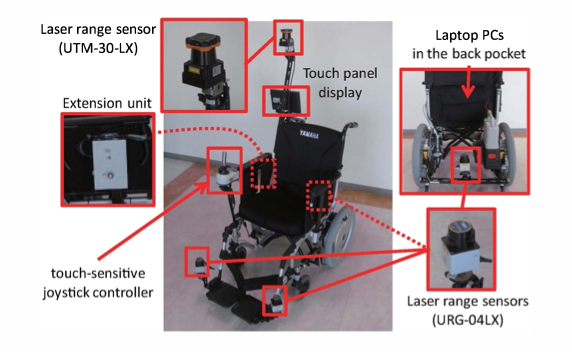
\includegraphics[height=60mm]{graphics/omni-vision wheelchair.png}
    \caption{Robotic Wheelchair with Omni-directional vision \cite{kobayashi_robotic_2012}.}
    \label{fig:omni-chair}
\end{figure}

The companion sets his/her initial position by tapping his/her facial image which is provided by the omni-directional camera.
The wheelchair has a laser range sensor, UTM-30LX by Hokuyo Electric Machinery, attached to a pole which is affixed to the wheelchair to be able to observe the upper body of the companion.
To observe the environment around itself it has 3 additional laser range sensors, URG-04LX. 
The wheelchair has an extension unit attached too the joystick controller to override the output signal generated by the software.
The lever of the joystick controller has been replaced with a touch-sensitive one so when the user touches the lever the control commands of the user override the signals from the software to ensure the safety of the user.

The wheelchair has three modes; side-following mode where the wheelchair is by the side of the companion, back-following mode where the wheelchair is behind the companion and insensitive mode where the wheelchair stops because the companion has stopped. 
The wheelchair desires to be in the side-following mode, but when the wheelchair senses that it can not be by its companion's side, it switches to the back-following mode until it is secure to return to the companion's side. 
The insensitive mode it entered when the chair senses that the companion has been stopped for 5 seconds and does not leave this mode until the companion is more than 80cm away from the wheelchair.
When leaving the insensitive mode the wheelchair goes to the back-following mode.
If the wheelchair loses his companion the system on the wheelchair can promptly re-identify the companion by using color appearances cues \cite{kobayashi_robotic_2012}.


\subsection{The Model H Hybrid}
Model H Hybrid as seen in figure \ref{fig:ModlHHybrid} is a true hybrid chair meaning that it can both be self-propelled by the user or use power to drive the motors so it can propel itself at any time.

\begin{figure}[!ht]
    \centering
    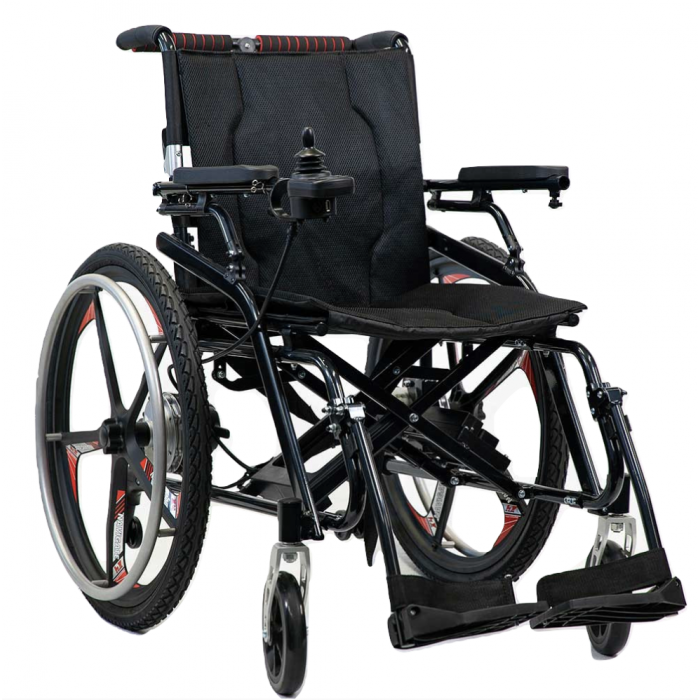
\includegraphics[height=55mm]{graphics/Hybrid_stóll.png}
    \caption{Model H Hybrid - The Hybrid Wheelchair \cite{jdy_imports_model_2022}.}
    \label{fig:ModlHHybrid}
\end{figure}

The chair is equipped with removable seat and seat belts, basic anti-tippers to prevent tipping forward or backwards, advanced lithium-ion batteries, a charger and 2 powerful motors to propel the wheelchair forwards or backwards should the user demand it. 
The batteries are 24V 6Ah lithium ion batteries. They give the wheelchair a range up to 8 miles or almost 13 km and a max speed of 5 mph or 8 km/h.
The chair itself is incredibly light or 39 lbs (17.7 kg) and can handle a maximum weight up to 240 lbs, roughly 109 kilos. 
It also comes with a joystick to control and move it around. The key feature in this specific design is that it is incredibly light, as talked about before, compering to other electric wheelchairs and they are proud to be the lightest mobility chairs on the planet.
They are also easily foldable and can fit into almost all vehicles which gives them a great competitive edge.
What this design lacks is the ability to follow its user should the user decide to stand up and walk a short distance given that the user is not fully paralyzed \cite{jdy_imports_model_2022}.


\subsection{Person following robot CNN}
This is a project that was done at York University, Toronto Canada, where students integrated stereo vision with a CNN Tracker for a person-following robot. The tracker is able to track a human in real time using an online convolutional neural network. The robot is able to follow the target around corners even when it is momentarily unseen by estimating and replicating the local path of the target.
The person following robot can be seen in Figure \ref{fig:follow-robot}

\begin{figure}[!ht]
    \centering
    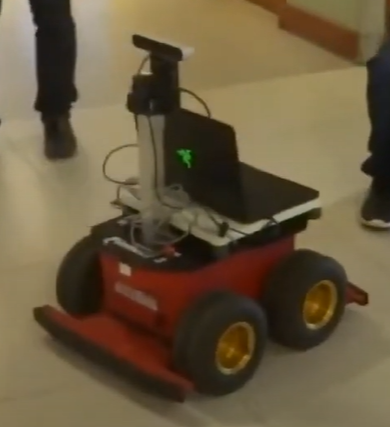
\includegraphics[height=60mm]{graphics/preson-following-robot.png}
    \caption{A person following robot with stereo vision based CNN tracker\cite{raghavender_sahdev_person_2017}.}
    \label{fig:follow-robot}
\end{figure}

The robot used is a Pioneer 3-AT robot, which is a small four-wheel, four-motor skid-steer robot ideal for all-terrain operation or laboratory experimentation. The Pioneer 3-AT comes complete with one battery, emergency stop switch, wheel encoders and a microcontroller with ARCOS firmware, as well as Pioneer SDK advanced mobile robotics software development package. 
The students equipped and tested this robot with two stereo cameras, the Point Grey Bumblebee2 from Teledyne Flir and the ZED stereo camera from Stereolabs, which act as the only sensors on the robot to sense its environment.
An online convolutional neural network (CNN) is used to track the given target under different situations, making use of RGB images and a stereo depth image for tracking, as well as a novel stereo dataset. A PID based controller is then used to steer in such a way so as to keep the target in the center of the image.
Possible future work includes incorporating dynamic obstacle avoidance
techniques with the person following robot to give it more intelligence.
